\chapter{Introduction}

\section{Background and motivation}
https://web.archive.org/web/20180830051336/https://www.rollingstone.com/music/music-news/nine-dead-at-pearl-jam-concert-235167/

On June 30th 2000, 9 young men passed away in a crowd crush during a Pearl Jam concert at Roskilde Festival in Denmark \cite{pearl_jam}. An uncontrolled surge, pushing the crowd towards the scene, caused immense pressure on the frontmost concert-goes, thrusting them against the barriers. The high-energy crowd unknowingly trampled the victims, who succumbed under the pressure of the crowd. This incident is unfortunately not the only one of its kind, as crowd crushes continue to occur at mass gatherings around the world.

\section{Crowd safety pain points}

\section{Brief history of Fluxense}

Together with two classmates, I founded Fluxense in January 2024.

\section{Scope and limitations}

\section{Problem statement}
\label{sec:problem-statement}

\section{Thesis structure}

Hubka and Eder (1995) characterize the design process as intuitive, iterative, innovative and unpredictable.

Process needs to organized. (citation?)

Blah blah, following product design methodology / frameworks. Many frameworks exist

\subsection{Comparison of frameworks}
\vspace{2em}
\begin{figure}[H]
  \centering
  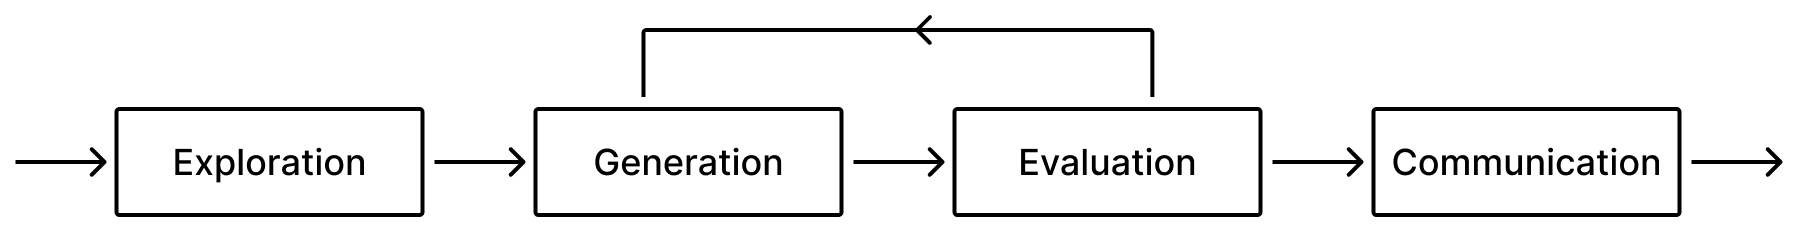
\includegraphics[width=14cm]{Pictures/Figures/cross.png}
  \caption{Cross' four-stage model of the design process}
  \label{fig:cross}
\end{figure}

Cross \cite{cross} proposes likely the most simplistic, yet well-known framework: a four-stage model comprised of \textit{exploration}, \textit{generation}, \textit{evaluation} and \textit{communication} (Figure \ref{fig:cross}). Cross describes this type of modal as descriptive, as it merely attempts to model the conventional, heuristic design process. More detailed models of this type exist, such as French's \cite{french} "anatomy of design," (Figure x) detailing four stages, most distinctly underlining the problem analysis and definition, as conducted in section \ref{sec:problem-statement}. According to Cross, these models differ from prescriptive models, which offer a more systematic procedure, as well an emphasis on analyzing and understanding the design problem before generating solution concepts. Perhaps the most well-known of these is offered by Pahl et. al \cite{pahl_beitz}, and is based on the following design stages: \textit{clarification of the task}, \textit{conceptual design}, \textit{embodiment design}, and \textit{detail design}. Combining the aforementioned models, Ulrich and Eppinger present a rather comprehensive framework. Their process is based on the following stages: \textit{concept development}, \textit{system-level design}, \textit{detail design}, and \textit{testing and refinement} \cite{ulrich_eppinger}.

These frameworks provide varying degrees of structure to the design process, but all share the commonality of being highly engineering-focused. In engineering a physical product, a rigid, structured process is often necessary as each iteration must be designed, manufactured and tested. This is costly, both in effort and material costs. Software, on the other hand, is much more flexible, with iterations being a magnitude faster and cheaper to develop. This demonstrates a need for adapting the design process to the context of the product being developed. Conveniently, Ulrich and Eppinger present a multitude of adaptations to their framework, including what they refer to as "Quick-Build Products" and "Digital Products." Here the \textit{detail design} and \textit{testing and refinement} stages are omitted, and replaced with a cyclical design-build-test process. Whereas the linear, rigid processes described previously are labelled as "waterfall methods", this iterative process is most often referred to as \textit{agile development}.

Agile development has a myriad of implementations, with the most popular being \textit{Scrum}. Scrum is based on the following stages: \textit{sprint planning}, \textit{daily stand-up}, \textit{sprint review}, and \textit{sprint retrospective}, with a sprint typically lasting 2-4 weeks \cite{scrum}.

Blah blah, these have engineering-focused prescriptive, software needs more flexibility, as explained by ulrich and eppinger, agile, scrum, double diamond





